\chapter{}

Em 7 de novembro de 1976, Paula nasceu, vinte dias antes do prazo.
O pai, que tanto esperara por ela, estava bem longe, plantando amendoim nas terras que comprara no interior de Goiás, num rincão em que as notícias só chegavam através do radinho de pilha de um caboclo morador do lugar.
Por sorte, o tal sujeito tinha por mania ouvir todas as manhãs o Nhô Zélio, um animador de programa de música caipira levado ao ar pela Rádio Cultura de Araraquara.
O jeito foi apelar para Nhô Zélio tentar fazer chegar ao pai a notícia do nascimento, o que o simpático artista fez com tanto empenho que não só o Paulo, mas toda a audiência do programa, que não era pequena, ficou sabendo.
Muitos amigos e conhecidos telefonaram em solidariedade, torcendo para que o aviso chegasse ao destino.

Paulo chegou suado, cansado, coberto de poeira, do jeito que descera do trator, assim que o caboclo foi anunciar-lhe o acontecido.
Subiu na caminhonete e veio, sem parar para nada, até bater na maternidade, tarde da noite, danado da vida porque a filha não esperara por ele.


\begin{figure}
\centering
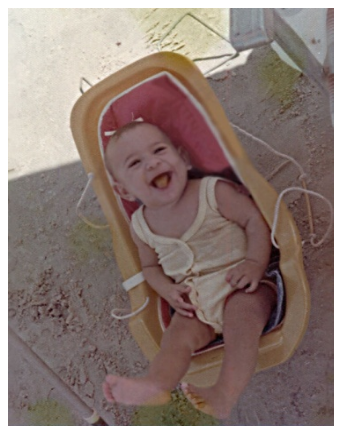
\includegraphics[width=0.6\linewidth]{26/paula-bebe.png}
\caption{Paula, o bebê mais risonho da casa.}
\end{figure}


\begin{figure}
\centering
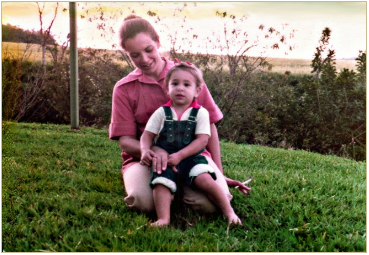
\includegraphics[width=0.6\linewidth]{26/paula-1o-ano.png}
\caption{Paula, no primeiro ano de vida.}
\end{figure}

Com quatro filhos agora, o magro salário da Casa da Lavoura, mesmo acrescido dos extras conseguidos com os projetos e vistorias para o banco, somados ainda ao meu ordenado de professora, não dava para nada.
Vivíamos no vermelho.
Com o dinheiro que esperava receber pela venda da Santa Teresa, Paulo tinha arrumado a fazenda para comprar em Goiás.
Demitiu-se da Casa da Lavoura e, visando fazer renda rapidamente é que decidiu plantar amendoim para produzir sementes selecionadas.

Certa vez, poucas horas depois de Paulo ter saído de viagem para a fazenda, um senhor telefonou e, identificando-se, perguntou pelo dono da plantação de amendoim que ele vira ao passar por aquelas paragens.
Quando lhe contei que ele estava justamente a caminho de lá, pediu-me com insistência que fizesse chegar ao Paulo os cumprimentos pela mais bonita plantação de amendoim que ele já vira, sobretudo naquela região que todos julgavam imprópria para essa cultura.

Todavia, como constataríamos meses mais tarde, aquele foi um péssimo ano para o amendoim.
Choveu torrencialmente na época da colheita e o amendoim perdeu-se quase todo, melado, como se diz.
Alguma outra saída precisava aparecer para nós, e com urgência.

Em toda a nossa história com o café no Mato Grosso, tivera importante participação Ludovico da Riva, um agrônomo saído também da Luís de Queiroz cujo pai, Ariosto da Riva, um veterano colonizador, começara sua saga de pioneiro no norte do Paraná, na primeira metade do século XX.
Foi Ludovico quem animou Paulo a plantar café na Bodoquena, indicou-nos a Santa Tereza, intermediou a venda da fazenda quando não pudemos mais mantê-la e, por fim, tornou-se um grande amigo do Paulo, mesmo apesar da enorme demora em nos pagar.

Durante o tempo em que se desenrolava a infindável liquidação da Santa Teresa, o velho Ariosto da Riva andava envolvido com um novo projeto de colonização bem ao norte do Mato Grosso, estimulado pelo enorme interesse dos governos militares na ocupação da Amazônia.
Muita gente, atraída pelo anúncio de generosos financiamentos e incentivos fiscais, começava a abrir grandes fazendas por lá, incluindo um tal Serafino Ferruzzi, um italiano muito rico, dono de uma das mais importantes frotas marítimas de transporte de grãos do mundo, grande proprietário de fábricas de cimento aqui no Brasil e que comprou, por intermédio do pai do Ludovico, uma extensa área próxima da cidadezinha de Alta Floresta, sede do projeto de colonização da família Da Riva.
O italiano cismara de plantar café nestas terras e procurava um agrônomo capaz de encarar o titânico desafio.
Ludovico pensou imediatamente em Paulo e falou dele para o pai, que o indicou ao empresário.
O salário era compensador e o trabalho exatamente do tipo capaz de galvanizar meu marido.
Dessa vez eu o apoiei, ainda que isso significasse levar praticamente sozinha a criação dos meninos, porque o Paulo só teria possibilidade de vir para casa a cada mês, mês e meio.

Meses depois de ter aceitado a empreitada, Paulo quis que eu fosse conhecer a Mogno, a fazenda do Ferruzzi.
Fui encontrá-lo em Cuiabá e, no dia seguinte, embarcamos num monomotor para Alta Floresta.
Cerca de uma hora de vôo mais tarde, deixávamos para trás a última grande área aberta na fímbria da floresta amazônica, a célebre Fazenda Mutum.
Daí por diante, prosseguiríamos ainda por hora e meia sobre a mata cerrada, sem vislumbrar uma única clareira, um fio de água, um esboço de estrada, um sinal de presença humana que fosse.
Perguntei ao piloto do pequeno avião:
\textit{``-- Comandante, o que o senhor faria se o motor começasse a falhar agora?''} 
\textit{``-- Escolheria uma castanheira bem forte e aterrissaria sobre ela''}, ele respondeu.

Pensei que fosse humor negro.
Não era.
\textit{``Mas''}, prosseguiu ele, tranquilizando-me, \textit{``não se preocupe; se você pudesse enxergar através da copa dessas árvores, ficaria espantada com o tanto de gente que circula aí embaixo.''}
\textit{``-- Índios?''}, eu quis saber.
Ele riu:
\textit{``Não.
Brancos.
Alguns até bem louros, de olhos azuis.
Missionários, contrabandistas de minérios, de bichos e plantas da Amazônia, madeireiros, garimpeiros, uma verdadeira correição de gente de todo o tipo.''}

Aterrissamos numa pista de terra, próximo do escritório da colonizadora, e seguimos de caminhonete para a fazenda.
Chegamos ao entardecer.
Fiquei impressionada.
A sede, uma grande construção de madeira, ficava no centro de uma clareira.
À volta, uma verdadeira muralha de vegetação, alta, escura e cerrada como eu nunca tinha visto, obstruía a visão e dava uma sensação claustrofóbica, acentuada pelo calor úmido que sufocava.
À noite, passada a hora dos mosquitos, saímos lá fora para experimentar o ar fresco que vinha da mata.
Dormimos enrolados numa manta leve.

Ao amanhecer, Paulo foi me mostrar as obras.
Mais uma vez, como em Bonito, pude me orgulhar da capacidade incrível do meu marido de comandar sozinho e perfeitamente à vontade um trabalho que empregava, naquele momento, cerca de mil trabalhadores ocupados em derrubar a mata, abrir a pista de pouso, estradas, construir pontes, levantar moradias e barracões para alojar escritório, oficina, serraria, secadores, enfermaria, refeitório.
Era um pequeno povoado que ali nascia para atender o projeto ambicioso do Dr.
Ferruzzi de plantar café e criar gado em terras da Amazônia.
Com o tempo, eu ainda haveria de me convencer daquilo que um fiel escudeiro do Paulo, o Zezinho, costumava afirmar a respeito do patrão:
\textit{``-- Quer ver o Paulo feliz é só arrumar para ele uma obra daquelas bem faraônicas!''}

\begin{figure}
\centering
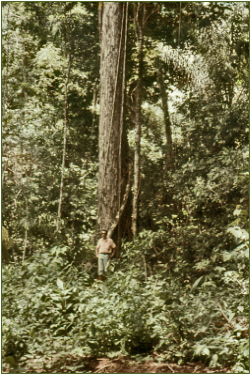
\includegraphics[width=0.6\linewidth]{26/paulo-no-mogno.png}
\caption{Paulo na floresta de mogno.}
\end{figure}

\begin{figure}
\centering
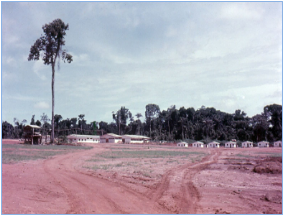
\includegraphics[width=0.6\linewidth]{26/obras-implantação.png}
\caption{As obras de implantação do projeto.}
\end{figure}

Terminada a implantação da Mogno, Paulo foi convidado a trabalhar com os Da Riva que abriam três fazendas em terras da colonizadora e pretendiam plantar cacau, café e pimenta-do-reino entre outras coisas, como demonstração das possibilidades que aquelas terras ofereciam aos que nelas viessem se estabelecer.
Então, fiz minha segunda viagem a Alta Floresta.
No avião, um garimpeiro distribuía entre as senhoras, alianças artesanais de ouro puro.
Ao descobrir que eu era mulher do Paulo, que ele conhecia, presenteou-me gentilmente com duas.

Diferentemente da Serra da Bodoquena, o lugar onde crescia a cidade de Alta Floresta não tinha sido anteriormente povoado de forma sistemática pelos civilizados.
O que havia por ali, como dissera o comandante do nosso avião, era um trânsito relativamente intenso de missionários, garimpeiros e aventureiros de toda a espécie que acabaram por espantar para longe as populações indígenas.
Ariosto Da Riva e sua colonizadora seriam pioneiros em começar um trabalho de fixação de uma população permanente na região.
E eu tive, por este motivo, o privilégio de viver uma experiência única naquele lugar: vi nascer uma cidade.

 Naqueles dias, acompanhando Paulo no seu trabalho, fui com ele a Paranaíta, um segundo polo de colonização que se seguiria a Alta Floresta.
Os colonos desta segunda área já estavam chegando e começavam a armar suas barracas de lona preta nos terrenos adquiridos da colonizadora.
Era como um cenário a se erguer num gigantesco estúdio cinematográfico ao ar livre: o lugar da farmácia, do hotel, da prefeitura, da delegacia, da igreja, era indicado por placas caprichosamente pintadas e distribuídas ao longo das ruas cascalhadas, segundo um plano diretor que o \textit{``Seu''} Ariosto nos mostrou orgulhoso.
Erguidas as barracas, armada a trempe do fogão, as famílias logo davam início à construção das suas casas de madeira.
Se eu voltasse poucos meses depois, veria uma pequena cidade pronta e funcionando como sua irmã mais velha, Alta Floresta.

Enquanto os grandes trabalhavam, a criançada se divertia, procurando no cascalho das ruas e das construções minúsculas pepitas de ouro.
A região era rica em ouro de aluvião e essa era a grande ameaça a ser enfrentada.
Uma noite, ouvimos de um sujeito que tinha terras lá perto que, pouco tempo atrás, ao abrir a janela pela manhã, dera com uma pequena multidão de cerca de trezentos garimpeiros apeando de caminhões na porteira da sua fazenda.
Correra um boato de que o rio que cortava a propriedade tinha muito ouro.
Garimpeiro, segundo ele, era como praga de gafanhotos; não há quem segure.
E, se por azar, encontram ouro mesmo, adeus trabalho, não tem peão que resista ao sonho da riqueza instantânea.
Vai todo mundo para a bateia.


Nas conversas de fim de tarde, no refeitório da colonizadora, sempre aparecia um jovem delegado para contar as histórias extraordinárias que diariamente testemunhava, geradas pela fortuna tão abundante quanto fugaz proporcionada pelo garimpo.
Como aquelas das universitárias de Belém, de Cuiabá e até de São Paulo, que nos fins de semana se enfiavam floresta adentro para se prostituir entre os garimpeiros e, na segunda-feira, restituídas à condição de moças de família, voltavam para suas casas carregando malas pejadas de saquinhos de ouro.
Ou a do famoso cantor popular que se apresentou num dos cabarés do garimpo e saiu de lá dia alto, carregado e afônico, porque a cada vez que tentava finalizar o \textit{show}, um dos garimpeiros sacudia diante dele um frasquinho de pepitas, incentivando-o a continuar.

Tudo o que eu via e ouvia configurava um mundo novo e extraordinário para mim.
Na verdade, Paulo queria que eu me deixasse seduzir por aquela terra e por aquela vida.
Era esse o objetivo daquela segunda viagem ao norte do Mato Grosso.
Ele queria que eu aceitasse a ideia de levar nossos filhos para viver com ele lá.
Meu antigo sonho de viver uma experiência completamente nova ao lado dele teria me feito topar de olhos fechados.
Mas, com as crianças, não.
Sempre me pareceu que o fato de ter sob minha guarda a vida desses meninos não me dava o direito de pôr em risco o futuro deles.

\textit{``-- E todos esses filhos de colonos?''}, perguntava ele.
\textit{``Acha que vão morrer ou virar índios pelo fato de viverem aqui?''} 

Mas eu não me deixava convencer.
Aquele lugar era novo demais, desprovido demais.
Na época das chuvas, durante meses, nem bujão de gás chegava.
Os aviões não decolavam ou não aterrissavam.
Os caminhões encalhavam.
Era tudo muito precário.
Que tipo de estudo poderíamos proporcionar-lhes ali? E se um deles ficasse doente? O socorro mais próximo estava em Cuiabá e sabe-se lá de que qualidade! Ainda uma vez, recusei e voltei para Araraquara.


No último dia em que fiquei lá, esperava pelo Paulo na porta do escritório, quando vi um jovenzinho chegar a pé pela estrada, como que a passeio.
Loirinho, de óculos, jeito de primeiro aluno da classe.
Perguntou-me pelo gerente da empresa.
Pedi-lhe que aguardasse, que Paulo logo viria.
Curiosa, quis saber como chegara até ali, uma vez que naquele dia não havia aterrissado avião algum na pista.
\textit{``-- De carona, num caminhão.''} 
\textit{``-- Vindo de onde?''}, perguntei.
 \textit{``-- De Santa Catarina''}, respondeu com simplicidade.
\textit{``-- Veio de Santa Catarina assim, de carona, o tempo todo?''}, insisti.
 
\textit{``-- Pois é''}, ele continuou, \textit{``tirei meu diploma de agronomia e ouvi dizer que estavam abrindo fazendas aqui; então eu vim para ver se arrumo um emprego.''}

Paulo arrumou-lhe o emprego.
Revelou-se um fitopatologista de primeira linha.
Mas a coisa mais formidável a respeito dessa criatura, meu marido contou-me mais tarde: em poucas semanas ele organizou um coro de crianças que cantava aos domingos na capela improvisada pelos colonos.
Um dia, muito tempo depois, ele iria embora para cursar uma pós-graduação.
Tornou-se professor da Universidade Federal do Mato Grosso.


Anos mais tarde, eu havia de aprender com gente como esse jovem, com meus próprios filhos e com muitos amigos dos meus filhos, que nestes rincões distantes do Brasil, exatamente pelos muitos obstáculos a superar, é que surgem extraordinários seres humanos e grandes histórias de vida.
 Mas, naqueles dias eu ainda não tinha vivência para acreditar nisso.

